\documentclass[12pt]{article}

\usepackage[utf8]{inputenc}
\usepackage[T1]{fontenc}
\usepackage{times}
\usepackage[textwidth=5.5in,textheight=9in]{geometry}
\usepackage{graphicx}
\usepackage{booktabs}
\usepackage{float}
\usepackage{amsmath,amsfonts}
\usepackage{xcolor}
\usepackage{hyperref}


\newcommand{\note}[1]{\textcolor{blue}{#1}}

\title{\vspace{-1em}\textbf{Evaluating Agents}\\
  \vspace{1em}
  \normalsize{\normalfont LLM Engineering Project Report}}

\author{
  Leonard Gruber \quad Lukas Gruber \quad Yassine Ajoud\\
}

\date{}

\begin{document}

\maketitle

\begin{abstract}
Agents built from LLMs are usually compared by task accuracy. In this project we test this. We built a small travel agent with a weather tool and a calculator and wrote 25 questions with known correct answers. Two models, Qwen2.5-0.5B-Instruct and Qwen2.5-1.5B-Instruct, answered the original questions and rephrased versions of them. We measured accuracy, tool use, robustness and efficiency. The larger model is more accurate (0.80 vs 0.64) but it often fails by refusing to call its weather tool on cleanly worded questions. The smaller model loses accuracy on rephrased questions (0.64 to 0.56) while the larger one does not.
\end{abstract}

\section{Introduction}
An LLM agent is a language model that can call tools in a loop. Benchmarks usually report task accuracy for an agent. The question behind our project comes straight from the project kickoff: "Is there more to agents than accuracy?"

We kept the setup small so we could control everything. Our agent is a travel assistant with two tools. The weather tool returns fixed values instead of live data, so every question has one known correct answer and every run can be repeated exactly. We compare two instruction tuned models of different size on 25 questions. Each question exists in a clean version and in a casual version with typos, like a real user would type it. For every run we log whether the answer is correct, which tools were called, how many model calls and tokens it needed and how long it took.

The headline number says the larger model is better: 0.80 against 0.64 accuracy. The interesting part is what sits behind the failures. The larger model refuses to call its weather tool on several cleanly worded questions but answers the casual versions of the same questions. The smaller model handles single tool calls well but breaks when a question needs two tool steps. None of this is visible in the accuracy number.

\section{Related Work}
There are many benchmarks for LLM agents and most of them work the same way. The agent gets a fixed set of tasks and the benchmark reports how many of them it solves. The tasks can be function calls, coding problems, web navigation or general assistant requests. Task accuracy is the standard number in most comparisons of agents.

Some recent work questions whether this one number is enough, because two agents with the same accuracy can still differ a lot in cost and in how reliably they behave across runs and phrasings. Our project follows this idea on a very small scale. Instead of a large benchmark we use a task set that is small enough to inspect every single run by hand.

\section{Approach}

\subsection{Agent loop}
We reuse the agent loop from the lecture. The model gets the user question plus a JSON schema for each tool. When the model writes a \texttt{<tool\_call>} block we parse it, run the matching Python function and append the result to the conversation as a tool message. Then the model is called again. The loop ends when the model answers without a tool call. After six iterations without a final answer the run counts as failed.

\subsection{Tools}
\texttt{get\_weather(city)} returns a fixed temperature for one of 16 cities, for example ``Tokyo: 26.0 degrees Celsius''. \texttt{calculator(expression)} evaluates a plain math expression. We use fixed weather data on purpose. The correct answers are known in advance and the runs can be repeated. The notebook also works offline this way.

\subsection{Tasks}
Table~\ref{tab:tasks} lists the 25 tasks. Tasks 1 to 9 need the weather tool, tasks 10 to 17 need the calculator and tasks 18 to 25 need both, for example for a temperature in Fahrenheit or for the difference between two cities. Every task has a rephrased variant for the robustness test, written the way a real user might type it, with casual wording and typos. Table~\ref{tab:variants} lists all of them. For example task 18 becomes ``My friend from the US asks how hot Cairo is right now, tell me in fahrenheit please''. The expected answer stays the same.

\begin{table}[H]
\centering
\footnotesize
\begin{tabular}{c p{2.9in} c l}
\toprule
\# & Question & Expected & Tools \\
\midrule
1 & What is the current temperature in Tokyo? & 26.0 & weather \\
2 & What is the current temperature in London? & 14.0 & weather \\
3 & How warm is it in Paris right now? & 21.0 & weather \\
4 & What is the temperature in Rome at the moment? & 29.0 & weather \\
5 & How cold is it in Oslo right now? & 8.0 & weather \\
6 & How hot is it in Dubai at the moment? & 41.0 & weather \\
7 & What is the current temperature in Sydney? & 23.0 & weather \\
8 & What is the temperature in Bangkok right now? & 33.0 & weather \\
9 & How cold is it in Reykjavik at the moment? & 3.0 & weather \\
10 & A hotel costs 120 euros per night. How much do 7 nights cost? & 840 & calculator \\
11 & I have 1000 euros for a 5 day trip. How much can I spend per day? & 200 & calculator \\
12 & Three museum tickets cost 24 euros each. How much do they cost together? & 72 & calculator \\
13 & The taxi cost 45 euros and the train ticket 82 euros. How much did I spend on transport? & 127 & calculator \\
14 & The flight costs 480 euros and the hotel 630 euros. How much is that together? & 1110 & calculator \\
15 & I plan to spend 85 euros per day for 14 days. How much do I need in total? & 1190 & calculator \\
16 & I had 300 euros for souvenirs and spent 137 euros. How much is left? & 163 & calculator \\
17 & A rental car costs 66 euros per day. How much do 6 days cost? & 396 & calculator \\
18 & What is the current temperature in Cairo in Fahrenheit? & 95.0 & weather, calculator \\
19 & How many degrees warmer is it in Berlin than in Moscow right now? & 13.0 & weather, calculator \\
20 & What is the current temperature in Madrid in Fahrenheit? & 87.8 & weather, calculator \\
21 & How many degrees warmer is it in Athens than in Toronto right now? & 18.0 & weather, calculator \\
22 & What is the current temperature in Toronto in Fahrenheit? & 53.6 & weather, calculator \\
23 & How many degrees warmer is it in Lisbon than in Oslo right now? & 16.0 & weather, calculator \\
24 & What is the average temperature of Sydney and Athens right now? & 26.5 & weather, calculator \\
25 & How many degrees warmer is it in Dubai than in London right now? & 27.0 & weather, calculator \\
\bottomrule
\end{tabular}
\caption{The 25 tasks with the expected answer and the expected tools.}
\label{tab:tasks}
\end{table}

\begin{table}[H]
\centering
\footnotesize
\begin{tabular}{c p{4.3in}}
\toprule
\# & Rephrased variant \\
\midrule
1 & Im packing for my trip, how warm is it in tokyo at the moment? \\
2 & Going to London tomorow, how many degrees is it over there? \\
3 & were heading to paris tomorow, hows the weather there, how warm? \\
4 & my sister wants to know how hot rome is right now \\
5 & packing for oslo, whats the temperature there now \\
6 & we land in dubai tonight, how hot is it there right now? \\
7 & quick question, how many degrees is it in sydney at the moment? \\
8 & whats the temp in bangkok right now, is it super hot? \\
9 & going to reykjavik next week, how cold is it there right now? \\
10 & We booked 7 nights in a hotel that charges 120 euros a night, what does that cost in total? \\
11 & me and my brother have 1000 euros for our 5 day trip, whats our daily budget? \\
12 & me and my 2 friends want museum tickets, 24 euros each, what do we pay together? \\
13 & taxi was 45 euros and the train 82, what did we spend on transport? \\
14 & flight is 480 and the hotel 630, how much is the trip so far? \\
15 & we plan 85 euros a day for two weeks, how much do we need in total? \\
16 & i had 300 euros for souvenirs and already spent 137, how much is left? \\
17 & rental car is 66 a day and we need it 6 days, whats the total? \\
18 & My friend from the US asks how hot Cairo is right now, tell me in fahrenheit please \\
19 & Is it warmer in Berlin or in Moscow at the moment, and by how many degrees? \\
20 & my us friend asks how warm madrid is right now, can you tell me in fahrenheit? \\
21 & is athens warmer than toronto right now and by how many degrees? \\
22 & whats the temperature in toronto at the moment in fahrenheit? \\
23 & how much warmer is lisbon than oslo right now? \\
24 & whats the average temperature of sydney and athens at the moment? \\
25 & how many degrees hotter is dubai than london at the moment? \\
\bottomrule
\end{tabular}
\caption{The rephrased variants of the 25 tasks. They keep the same expected answer but sound like a real user.}
\label{tab:variants}
\end{table}

\subsection{Metrics}
\begin{itemize}
\item \texttt{correct}: the final answer contains the expected number. We allow a tolerance below 1.0 for rounding.
\item \texttt{right\_tools}: the set of tools the agent called is exactly the expected set. We keep this separate from correctness because a model can reach the right answer without the expected tools and it can also call the right tools and still fail.
\item Cost: model calls, tool calls, generated tokens and seconds per run.
\end{itemize}

\subsection{Example run}
This is what a single run looks like. The 1.5B model gets the question ``What is the current temperature in Tokyo?'' and does not answer directly. Instead it writes a tool call:

\begin{verbatim}
<tool_call>
{"name": "get_weather", "arguments": {"city": "Tokyo"}}
</tool_call>
\end{verbatim}

We run the function and it returns ``Tokyo: 26.0 degrees Celsius''. This string goes back to the model as a tool message. The model then writes its final answer: ``The current temperature in Tokyo is 26.0 degrees Celsius.'' It finds the expected 26.0 in the answer and marks the run as correct. The whole run needed two model calls, one tool call and 36 generated tokens. Since the model can only know the value 26.0 from the tool, a correct answer tells us that the whole chain worked.

\section{Experiments}

\subsection{Data}
We did not use an external dataset. The 25 tasks and their variants are our data (Table~\ref{tab:tasks}). Writing them ourselves means we control the ground truth and can keep the tool data consistent with the expected answers.

\subsection{Evaluation method}
Accuracy is the share of solved tasks out of 25. The robustness number is the same accuracy measured on the rephrased variants. The tool score is the share of runs with exactly the expected tool set. The cost numbers are averages over the 25 original runs.

\subsection{Experimental details}
We use Qwen2.5-0.5B-Instruct and Qwen2.5-1.5B-Instruct with the transformers library, loaded in bfloat16. Decoding is greedy, so every run is deterministic. A model call generates at most 256 new tokens and a run stops after at most 6 loop iterations. All experiments ran on a laptop CPU. The full evaluation, 100 agent runs, takes around 35 minutes.

\subsection{Results}
Table~\ref{tab:results} shows the results. The 1.5B model solves 20 of 25 original questions, the 0.5B model 16 of 25. On the rephrased variants the 0.5B model drops to 14 of 25 while the 1.5B model reaches 21 of 25 (Figure~\ref{fig:acc}). The 1.5B model needs fewer tokens per task but is more than twice as slow per run on our CPU.

\begin{table}[H]
\centering
\small
\begin{tabular}{lcccccc}
\toprule
Model & Acc. & Acc. (reph.) & Right tools & Model calls & Tokens & Seconds \\
\midrule
Qwen2.5-0.5B & 0.64 & 0.56 & 0.64 & 1.92 & 67.0 & 9.2 \\
Qwen2.5-1.5B & 0.80 & 0.84 & 0.68 & 1.84 & 52.9 & 22.1 \\
\bottomrule
\end{tabular}
\caption{Results. Accuracy on the original and the rephrased questions, share of runs with exactly the expected tools and average cost per run on the original questions.}
\label{tab:results}
\end{table}

\begin{figure}[H]
\centering
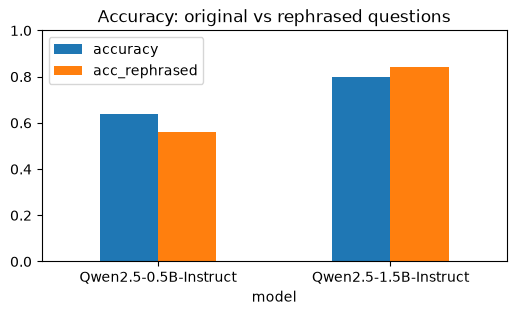
\includegraphics[width=0.75\linewidth]{accuracy.png}
\caption{Accuracy per model on the original and the rephrased questions.}
\label{fig:acc}
\end{figure}

\section{Analysis}
On four of the eight two-tool questions the 1.5B model did not call any tool and failed. For the Cairo question it answered that it has no access to live weather data, although the weather tool was listed right in its prompt. On the rephrased set the same model reaches 0.84, so several of these refusals disappear when the wording is casual. The wording decides whether the tools get used at all.

The 0.5B model fails differently. It is solid on single tool calls (8 of 9 weather questions, 6 of 8 calculator questions) but breaks on chains. On the Fahrenheit questions it returned the Celsius value and stopped. On two calculator questions it wrote a broken expression, got an error back and answered from the error text instead of fixing the call.

Right answers without the expected tools happen on both sides. The 0.5B model solved two temperature comparisons with two weather calls and mental subtraction. The 1.5B model computed 85 times 14 in its head without the calculator and converted Toronto to Fahrenheit right after a single weather call. These runs count as correct but fail the tool check. That is why the tool scores (0.64 and 0.68) tell a different story than the accuracies.

Rephrasing hurt the small model (0.64 to 0.56) and helped the large one (0.80 to 0.84). We expected typos and casual wording to make everything harder. For the 1.5B model the opposite is true.

On cost the 1.5B model uses fewer tokens per task (52.9 against 67.0) and slightly fewer model calls, partly because a refused run ends after one call. In wall clock time it is much slower on our CPU (22.1s against 9.2s per task on average).

\section{Conclusion}
We compared two Qwen2.5 models as tool-using agents on 25 travel questions with known answers and we measured more than accuracy. The larger model wins on accuracy but its failures have a pattern that accuracy does not show. It often refuses tool calls on cleanly worded questions. The smaller model fails differently. It breaks when a question needs two tool steps.

The setup has clear limits. 25 tasks, one paraphrase per task and two small models allow no general claims and our grader only checks numbers, so it cannot judge free text. Within these limits the answer to the project question is yes. There is more to agents than accuracy and without tool use, robustness and cost we would have misread both models.

\section*{Author contribution statement}
We planned the project together. All three authors worked on the code, the experiments and the report.

\section*{GenAI use}
We used Claude and ChatGPT during this project to generate simple functions and refine them. It helped with debugging the notebook code. We also used DeepL to translate and rewrite some sentences in the report. We reviewed the code and the text and checked it.

% \section*{References}
% references will be added here

\end{document}
